% CHAPTER START
The Trigger/DAQ system sends and saves data from the detector to a persistent data storage solution.
It's at this stage where the data isn't yet ready for an effective analysis, so what needs to happen is the data needs to be reconstructed and consolidated into physics objects, or Analysis Object Data (AOD) files.
Creating AODs from data requires significant computation power and Athena is the software framework that plays a significant role in this process.
This chapter will cover the software tools used by ATLAS 

\section{Athena and ROOT}
% \subsection{What is Athena}
Athena is the open-source software framework for the ATLAS experiment.\cite{athena}
It uses on other software such as ROOT, Geant4 and other software as part of the LCG software stack. 
Athena manages ATLAS production workflows which include event generation, simulation of data, reconstruction from hits, and derivation of reconstructed hits.\cite{athenadocs}
It also provides some in-house based analysis tools as well as tools for specifically ROOT based analysis.

ROOT is an open-source software framework used for high-energy physics analysis at CERN.\cite{ROOT_about} 
It uses C++ objects to save, access, and process data brought in by the various experiments based at the LHC, the ATLAS experiment uses it in conjunction with Athena.
ROOT largely revolves around organization and manipulation of TFiles and TTrees into ROOT files.

\subsection{Continuous Integration (CI) and Development}
CI is a software development practice where new code is tested and validated upon each merge to the main branch of a repository. 
Every commit to the main branch is automatically built and tested for specific core features that are required to work with the codebase. 
This helps to ensure that the codebase is working as intended and that the new code is compatible with the existing codebase.

Athena is developed with CI by using an instance of Jenkins, called ATLAS Robot, to build and test the new changes within a merge request interface. 
ATLAS Robot will then provide a report of the build and test results.
If the build or test fail, ATLAS Robot will provide a report of which steps failed and why.
This allows for early detection of issues before the nightly build is compiled and tested.



\section{TTree Object} \label{section: ATLASIO_TTreeObject}
A TTree is a \verb|ROOT| object that organizes physically distinct types of event data into branches.
Branches hold data into dedicated contiguous memory buffers, and those memory buffers, upon compression, become baskets.
These baskets can have a limited size and a set minimum number of entries. 
The Athena default basket size at present is 128 kB, and the default minimum number of entries is 10. 

One function relevant to TTree is \verb|Fill()|. 
\verb|Fill()| will loop over all of the branches in the TTree and compresses the baskets that make up the branch.
This removes the basket from memory as it is then compressed and written to disk.
It makes reading back branches faster as all of the baskets are stored near each other on the same disk region. \cite{ROOT_TTree}

% AutoFlush
\verb|AutoFlush| is a function that tells the \verb|Fill()| function after a designated number of entries of the branch, in this case vectors, to flush all branch buffers from memory and save them to disk. 


\section{Derivation Production Jobs}
A derivation production job takes AODs, which comes from the reconstruction step at $\mathcal{O}(1 \text{ MB})$ per event, and creates a derived AOD (DAOD) which sits at $\mathcal{O}(10 \text{ kB})$ per event.
Derivation production is a necessary step to make all data accessible and useful for physicists doing analysis.
While derivations are reduced AODs, they often contain additional information useful for analysis, such as jet collections and high-level discriminants.\cite{PHYSLITE_A_new_2024}
Athena provides two types of output files from a derivation job, PHYS and PHYSLITE. 
PHYSLITE being the smallest file of the two, sees the largest effect upon attempts of optimization. 
These jobs can demand heavy resource usage on the GRID, so optimization of the AOD/DAODs for derivation jobs can be vital. 

\begin{figure}[h]
    \centering
    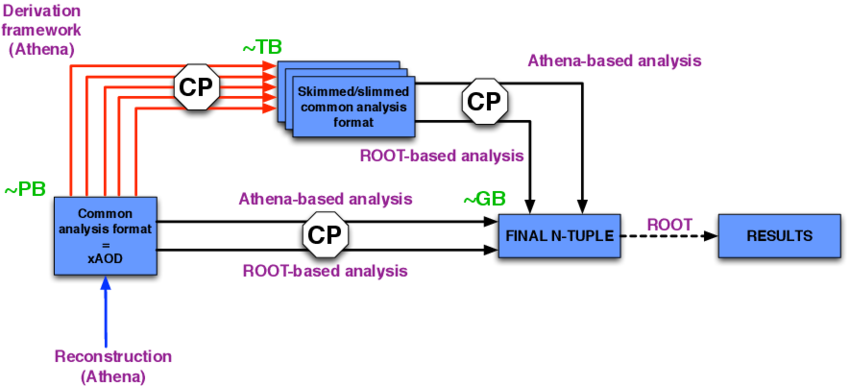
\includegraphics[width=0.8\textwidth]{content/img/catmore-derivation.png}
    \caption{Derivation production from Reconstruction to Final N-Tuple\cite{DAOD_Laycock_2014}}
    \label{fig:IO_derivation_framework}
\end{figure}

The derivation framework is sequence of steps that are performed on the AODs to create the DAODs.
Skimming is the first step in the derivation framework, and it's responsible for removing whole events based on pre-defined criteria.
Thinning is the second step, and it removes whole objects based on pre-defined criteria.
Lastly slimming removes variables from objects uniformly across events. 


\section{Event Data Models}
% \subsection{What is an Event Data Model}
An Event Data Model (EDM) is a collection of classes and their relationships to each other that provide a representation of an event detected with the goal of making it easier to use and manipulate by developers.
An EDM is how particles and jets are represented in memory, stored to disk, and manipulated in analysis.
It's useful to have an EDM because it brings a commonality to the code, which is useful when developers reside in different groups with various backgrounds.
An EDM allows those developers to more easily debug and communicate issues when they arise.  

\subsection{Transient/Persistent (T/P) EDM}
One of the previous EDM schemas used by ATLAS concerned a dual transient/persistent nature of AOD.
The AOD at this point was converted into an ntuple based format called D3PDs. 
While this conversion allowed for fast readability and partial read for effient analysis in ROOT, it left the files disconnected from the reconstruction tools found in Athena.\cite{Athena_xAOD_design}
The transient data was present in memory and could have information attatched to the object, this data could gain complexity the more it was used.
Persistent data needed to be simplified before it could be persistified into long-term storage (sent to disk). 
ROOT had trouble handling the complex inheritance models that would come up the more developers used this EDM. 
Before the successor to the T/P EDM was created, ATLAS physicists would convert data samples using the full EDM to a simpler one that would be directly readable by ROOT.
This would lead to duplication of data and made it challenging to develop and maintain the analysis tools to be used on both the full EDM and the reduced ones.
Additionally, converting from transient to persistent data was an excessive step which was eventually removed by the adoption of using an EDM that blends the two stages of data together, this was dubbed the xAOD EDM.




\subsection{xAOD EDM}
The xAOD EDM is the successor to the T/P EDM and brings a number of improvements.
This EDM, unlike T/P, is usuable both on Athena and ROOT.
It's easier to pick up for analysis and reconstruction. 
xAOD EDM has the ability to add and remove variables at runtime, these variables are called ``decorations."

